\begin{figure}[!ht]
\centering
\begin{subfigure}[h]{0.8\columnwidth}
\centering
\epsfig{file=slidingwindow1.eps,width=1.2\columnwidth}
\caption{Step 1}
\label{fig:sw1}
\end{subfigure}
%\myskip
\begin{subfigure}[h]{0.8\columnwidth}
\centering
\epsfig{file=slidingwindow2.eps,width=1.2\columnwidth}
\caption{Step 2}
\label{fig:sw2}
\end{subfigure}
%\myskip
\begin{subfigure}[h]{0.8\columnwidth}
\centering
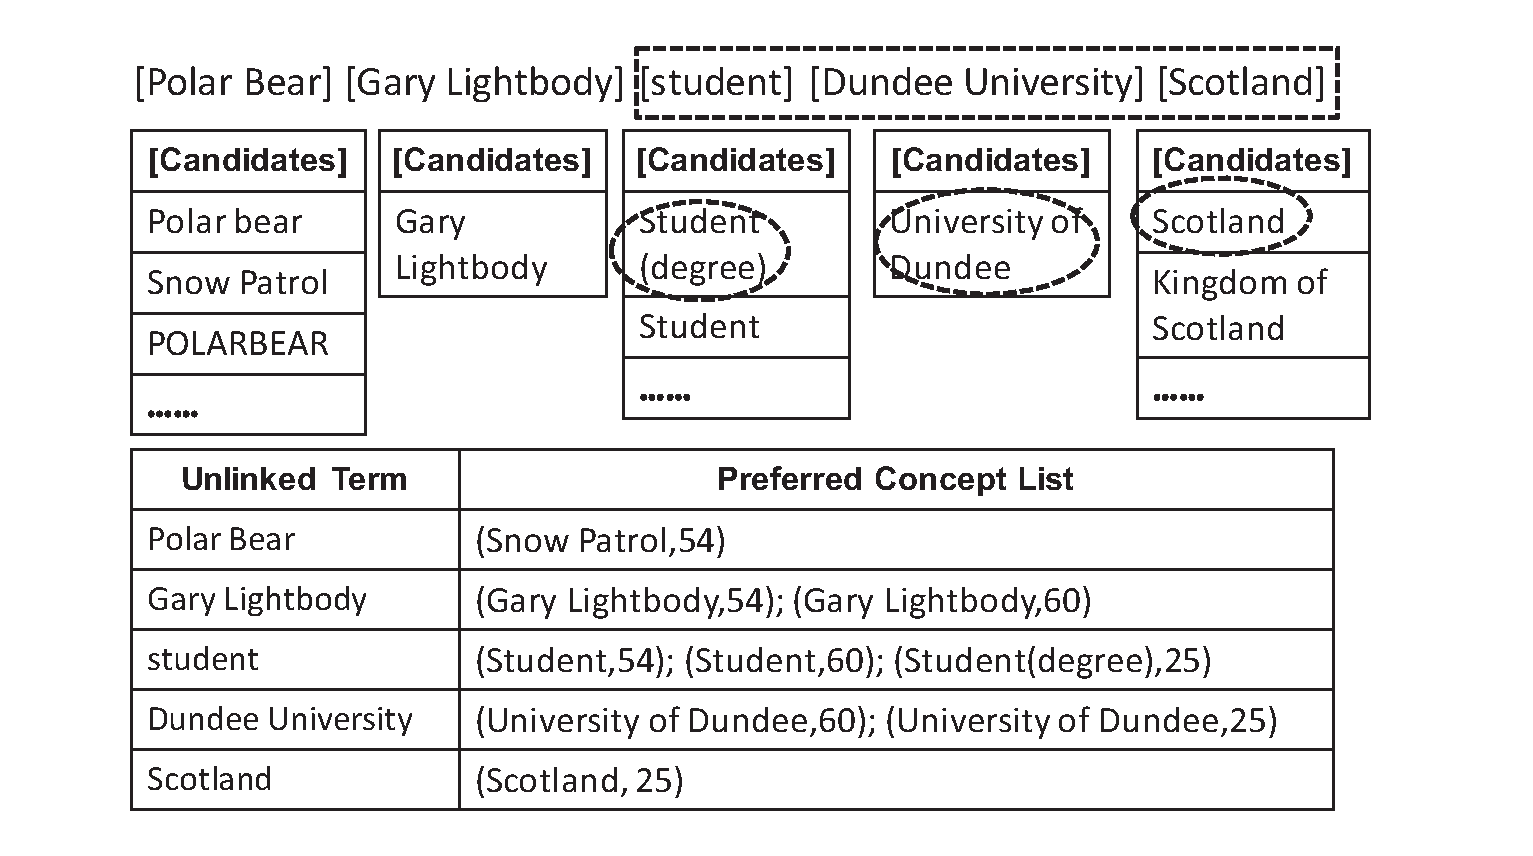
\epsfig{file=slidingwindow3.eps,width=1.2\columnwidth}
\caption{Step 3}
\label{fig:sw3}
\end{subfigure}
\caption{Sliding Window Example}
\label{fig:sw}
\end{figure}

\subsection{Wikify New Documents}
\label{sec:wikify}


%With the final co-occurrence matrix and appearance frequency of concepts generated after iteration,
%we can start our wikification process.
To wikify an entire document, our general idea is to
disambiguate several unlinked terms together within
a local context by optimizing the likelihood of co-occurrence among
a particular combination of senses for these terms. We could use
the whole document as the context but that will be computationally infeasible if
the document is large.
Instead we make the size of the context parameterized and tunable.
However, a local context can be misleading and can introduce errors in the
disambiguation. We solve this problem by creating a sliding window
that allows us to aggregate the disambiguation results from neighboring contexts
together and then make a pseudo-global decision about which sense each term
ultimately should have.

%What's
%different from the parsing result of Wikipedia corpus we use in the co-occurrence matrix enrichment
%phase is that this time we just have one kind of terms, which is unlinked term. All terms we
%recognize using our parser have a candidate Wikipedia concept list.
%All terms from the parse are unlinked terms.
%Unlike the enrichment phase, we have no linked term to help distinguish senses of the unlinked terms. So we come up with a method that uses the co-occurrence between candidate concepts to support
%one candidate concepts combination. To better explain our method, we first give some annotations here.

We illustrate this idea using \exref{ex-bear2} and show three steps
in sliding a window of size three in \figref{fig:sw}.
We parse the plain text using the NLP chunker discussed in Algorithm \ref{parsechunk}
and get the following terms: ``Polar Bear'', ``Gary Lightbody'', ``student'',
``Dundee University'' and ``Scotland''.
We create a candidate sense list for each term. Step 1 shows a window
containing ``Polar Bear'', ``Gary Lightbody'' and ``student''. Given that
each term has a few senses as candidates,
there are many combinations of senses for these three terms, such as:
\begin{itemize}
\item Polar bear, Gary Lightbody, Student (degree)
\shrink\item Snow Patrol, Gary Lightbody, Student
\shrink\item POLARBEAR, Gary Lightbody, Student (degree)
\end{itemize}
{\em Snow Patrol}, {\em Gary Lightbody} and {\em Student} turn out to be
the best sense combination since the sum of the {\em pair-wise}
co-occurrence is the largest at 54. Note here that we are simulating
the overall co-occurrence with pair-wise co-occurrence, which is a reasonable
approximation under computation constraints. We call the maximum sum
{\em sliding window score} ($S_{SW}$), and every term within this window
is associated with this disambiguation result (in the form of sense-$S_{SW}$ pair)
in a data structure called {\em Preferred Concept List} ($PCL$).

In Step 2, the window is slided to the right by one term, and the best
combination of senses is again computed while the $PCL$ is updated with three
more entries. This time $S_{SW}$ is 60.

In Step 3, within the last window of this sentence. The best combination
contains the {\em Student (degree)} sense, which is different from the result
of ``student'' in the 2 previous steps.

After we have finished sliding the window from start to finish, we group
the results for each term by senses and sum the $S_{SW}$ by the group.
In the case of ``student'', {\em Student} sense has a combined $S_{SW}$ of
114 while {\em Student (degree)} sense has a combined $S_{SW}$ of 25. The
first sense wins and becomes the final sense for the term ``student''.
Other terms are similarly disambiguated.

The detailed sliding window wikification algorithm is given in Algorithm
\ref{slide}. $L_u$ stands for the list of unlinked terms. $W_s$ stands for the
size of the sliding window. By picking one concept for each unlinked terms inside
the sliding window, we get a \emph{Concept Combination} ($CC$). 
Picking different candidate concepts from unlinked terms 
gives different $CC$s, thus forms the \emph{Concept Combination List} ($CCL$).
Therefore, $S_{SW}$ can be defined as
\[
S_{SW}=\max_{CC\in CCL}\sum_{c_i,c_j\in CC;i\neq j}{Co\left(c_i,c_j\right)}
\]
The $CC$ associated with $S_{SW}$ is called \emph{Best Concept Combination} ($BCC$).
$PCL_{L_u[i]}$ denotes the $PCL$ of the $i$th term in $L_u$.
%
%
%After parsing, we get a list of unlinked terms which represent the whole
%document, and it is denoted as $L_{T_u}$.
%We create a {\em sliding window} of $W_s$ consecutive terms. $W_s$ is the
%windows size which should not be confused with $W_c$ in \secref{sec:enrich}.
%The sliding window of terms basically create a segment of the article in which
%we try to disambiguate {\em all} the constituent terms together by maximizing a
%{\em sliding window score} (SWS). SWS is the sum of pair-wise concept
%co-occurrences.
%
%
%Each unlinked term $T_u$ in $L_{T_u}$ is associated
%with a data structure called \emph{Preferred Concept List}
%which is annotated as $PCL_{T_u}$. Each element in $PCL_{T_u}$ is a pair
%of a concept and a score known as {\em sliding window score} (SWS).
%
%When starting to wikify $T_u$ in $L_{T_u}$,
%we first pick the first $N$ terms from $L_{T_u}$.
%$N$ here is a parameter to set the size of the window containing all the currently handling terms. Not to confuse with the window
%we use in the matrix enrichment phase, we call this window \emph{Sliding Window}. By picking one
%candidate concept from each term in the sliding window, we get a combination of concepts with
%size $N$. We list all of the combinations of concepts in the sliding window.
%%We continue picking candidate concepts and finally get a list of combinations.
%The size
%of this list will be the product multiplied by the numbers of candidate concepts of all the terms in the
%sliding Window. We calculate a score for each combination by summing the co-occurrence frequency
%between each pair of candidate concepts. We sort the combination list by this score and pick up the
%rank 1 combination. In this combination, each term $T_u$ in the window has a chosen candidate concept.
%We then insert this chosen concept and the score of this combination to $PCL_{T_u}$.
%After updating of $PCL$, we slide the window one step forward to pick $N$ new terms and continue the process
%above, until we reach the end of $L_{T_u}$. Until now, each $T_u$ in $L_{T_u}$ has $PCL_{T_u}$ that
%may contain several elements. These elements are inserted when the sliding window move to
%different positions. Also, some elements may have the same concept. We scan the elements in $PCL_{T_u}$
%to calculate the score of each individual concept. The score of the same concept in different elements
%will be summed together. After that, we link $T_u$ to the concept with the highest score in $PCL_{T_u}$. However, if the highest score is 0, $T_u$ won't be assigned a link.
%When all the concepts of $T_u$ in $L_{T_u}$ are determined, the wikification process is done.

\begin{algorithm}[th]
\caption{Sliding Window Method}
\label{slide}
\begin{algorithmic}[1]
\Procedure{SlidingWindow}{$L_u$,$W_s$}
\For {$i \leftarrow 0,sizeof(L_u)-W_s$}
\State $CCL \leftarrow getCombination\left(L_u[i],W_s\right)$
\State Calculate $S_{SW}$ and $BCC$
%\State $BCC \leftarrow argmax_{CC\in CCL}\left(S_{SW}\left(CC\right)\right)$
\For {$j \leftarrow 0,sizeof(BCC)-1$}
\State Add $\langle BCC[j],S_{SW}\rangle$ to $PCL_{L_u[i+j]}$
\EndFor
\EndFor
\For {$i \leftarrow 0,sizeof(L_u)-1$}
\State Initialize $hash[concept \rightarrow score]$
\For {$j \leftarrow 0,sizeof(PCL_{L_u[i]})-1$}
\State $\langle key,value\rangle \leftarrow PCL_{L_u[i]}[j]$
%\If {$hash\;\;contain\;\;value$}
\State $hash[key] \leftarrow hash[key]+value$
%\Else
%\State $hash\left(key\right) \leftarrow value$
%\EndIf
\EndFor
\State $concept \leftarrow argmax_{key}\left(hash[key]\right)$
\If {$hash[concept]>0$}
\State Assign $concept$ to $L_u[i]$
\EndIf
\EndFor
\EndProcedure
\end{algorithmic}
\end{algorithm}

%\figref{fig:sw} shows a demonstration of the wikification process, taking the sentence we discuss in
%\secref{intro} as an example. After parsing, there are five unlinked terms recognized. Each unlinked term
%has a candidate concept list as is shown in \figref{fig:sw1}.
%The size of the sliding window is set to be 3. So in the first step of this process, the first
%three unlinked terms are taken into account.
%
%Then the $PCL$s of the first three terms are updated. ``Snow Patrol'' and the score 54 is inserted to the $PCL$
%of the first term. The updating of the other two terms are similar. After updating, we slide the window one step forward
%as is shown in \figref{fig:sw2}. This time, combination of ``Gary Lightbody'', ``Student'' and
%``University of Dundee'' is the best with score 60. Then the $PCL$s of the corresponding terms are updated.
%We continue slide the window until the last term is reached. After that, we scan the $PCL$ of each term to choose
%the best Wikipedia concept for it. Take ``Student'' as an example, the elements in its $PCL$ are:
%\begin{itemize}
%\item Student, 54
%\item Student, 60
%\item Student(degree), 25
%\end{itemize}
%The first two elements are of the same concept, so we sum the scores together. Then in ``Student'''s candidate
%concept list, ``Student'' has score 114, ``Student(degree)'' has score 25, others 0, so ``Student'' is chosen.
%
%Pseudo code is shown in Algorithm \ref{slide}.
%
